%
% fig-raender.tex
%
% (c) 2026 Prof Dr Andreas Müller
%
\begin{figure}
\centering
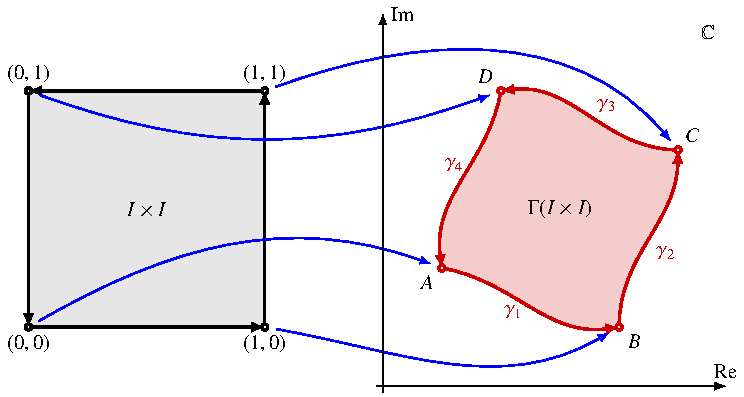
\includegraphics{chapters/030-integration/images/raender.pdf}
\caption{Zweidimensionale Kette und Rand.
\label{buch:integration:homologie:fig:raender}}
\end{figure}
